\chapter{Expertise and Memory}\label{s:memory}

\begin{objectives}

\item Define expertise and explain how it works using a graph metaphor
  for cognition.

\item Explain the difference between repetition and deliberate
  practice.

\item Define and construct concept maps, and explain the benefits of
  externalizing cognition.

\item Differentiate long-term and short-term memory, describe the
  capacity limits of the latter, and explain the impact of these
  limits on teaching.

\end{objectives}

\begin{quote}

  Memory is the residue of thought. \\
  --- Dan Willingham

\end{quote}

The previous chapter explained what distinguishes novices from
competent practitioners. This one looks at expertise: what it is, how
people acquire it, and how it can be harmful as well as helpful.  It
then shows how concept maps can be used to figure out how to turn
knowledge into lessons.

To start, what do we mean when we say someone is an expert? The usual
answer is that they can solve problems much faster than people who are
``merely competent'', or that they can recognize and deal with cases
where the normal rules don't apply. They also somehow make this look
effortless: in many cases, they instantly know what the right answer
is \cite{Parn2017}.

Expertise is more than just knowing more facts: competent
practitioners can memorize a lot of trivia without any noticeable
improvement in their performance. Instead, imagine for a moment that
we store knowledge as a network or graph in which facts are nodes and
relationships are arcs. (This is definitely \emph{not} how our brains
work, but it's a useful metaphor.) The key difference between experts
and competent practitioners is that experts' mental models are much
more densely connected, i.e., they are much more likely to know of a
connection between any two randomly-selected pieces of information.

\newpage % PDF

This metaphor helps explain many observed aspects of expert behavior:

\begin{itemize}

\item
  Experts can jump directly from a problem to its solution because there
  actually is a direct link between the two in their mind. Where a
  competent practitioner would have to reason ``A, B, C, D, E'', the
  expert can go from A to E in a single step. We call this
  \emph{intuition}, and it isn't always a good thing: when asked to
  explain their reasoning, experts often can't, because they didn't
  actually reason their way to the solution---they just recognized it.

\item
  Densely-connected graphs are also the basis for experts'
  \glossref{g:fluid-representation}{fluid representations}, i.e.,
  their ability to switch back and forth between different views of a
  problem \cite{Petr2016}. For example, when trying to solve a problem
  in mathematics, an expert might switch between tackling it
  geometrically and representing it as a set of equations to be
  solved.

\item
  This metaphor also explains why experts are better at diagnosis than
  competent practitioners: more linkages between facts makes it easier
  to reason backward from symptoms to causes. (And this in turn is why
  asking programmers to debug during job interviews gives a more
  accurate impression of their ability than asking them to program.)

\item
  Finally, experts are often so familiar with their subject that they
  can no longer imagine what it's like to \emph{not} see the world
  that way. As a result, they are often less good at teaching the
  subject than people with less expertise who still remember learning
  it themselves.

\end{itemize}

The last of these points is important enough to have a name of its
own: \glossref{g:expert-blind-spot}{expert blind spot}.  As originally
defined in \cite{Nath2003}, it is the tendency of experts to organize
explanation according to the subject's deep principles, rather than
being guided by what their learners already know.  While it can be
overcome with training, it's part of why there is no correlation
between how good someone is at doing research in an area and how good
they are at teaching it \cite{Mars2002}.

\begin{callout}{The J Word}

  Experts often betray their blind spot by using the word ``just'' in
  explanations, as in, ``Oh, it's easy, you just fire up a new virtual
  machine and then you just install these four patches to Ubuntu and
  then you just re-write your entire program in a pure functional
  language.''  As we discuss in \chapref{s:motivation}, doing this
  signals that the speaker thinks the problem is trivial and that the
  person struggling with it must therefore be stupid.

  Don't do this.

\end{callout}

\section{Concept Maps}\label{s:memory-concept-maps}

The graph metaphor explains why helping learners make connections is
as important as introducing them to facts: without those connections,
it's hard for people to recall things that they know.  To use another
analogy, the more people you know at a party, the less likely you are
to leave early.

Our tool of choice for representing someone's mental model as a graph
is a \glossref{g:concept-map}{concept map}, in which facts are bubbles
and connections are labelled arcs. It is important that they are
labelled: saying ``X and Y are related'' is only helpful if we explain
what the relationship \emph{is}. And yes, different people can have
different concept maps for the same topic, but one of the benefits of
concept mapping is that it makes those differences explicit.

As an example, \figref{f:memory-seasons} reproduces a concept map
taken from the \href{https://cmap.ihmc.us/}{IHMC CMap site} showing
why the Earth has seasons, and \figref{f:online-screencasting} uses a
concept map to explain how to create a good screencast.

\begin{figure}
\centering
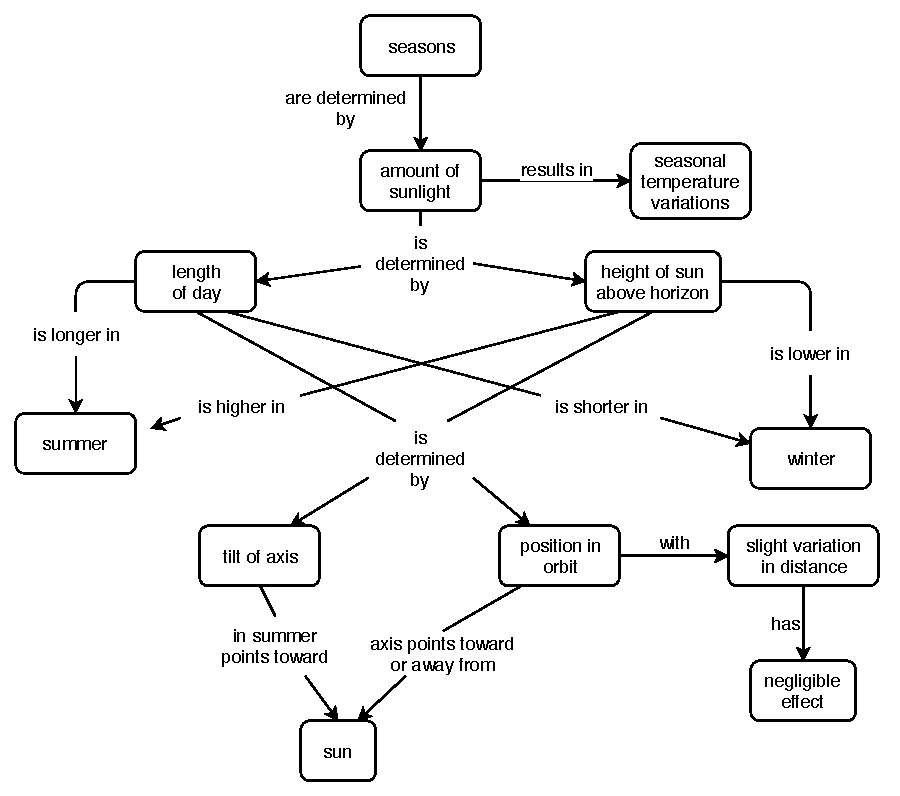
\includegraphics{../docs/fig/seasons.pdf}
\caption{Concept Map for Seasons (from \url{https://cmap.ihmc.us/})}
\label{f:memory-seasons}
\end{figure}

To show how concept maps can be using in teaching programming,
consider this \texttt{for} loop in Python:

\begin{verbatim}
for letter in "abc":
    print(letter)
\end{verbatim}

\noindent
whose output is:

\begin{verbatim}
a
b
c
\end{verbatim}

\noindent
The three key ``things'' in this loop are shown in the top of
\figref{f:memory-loop}, but they are only half the story.  The
expanded version in the bottom shows the \emph{relationships} between
those things, which are as important for understanding as the concepts
themselves.

\begin{figure}
\centering
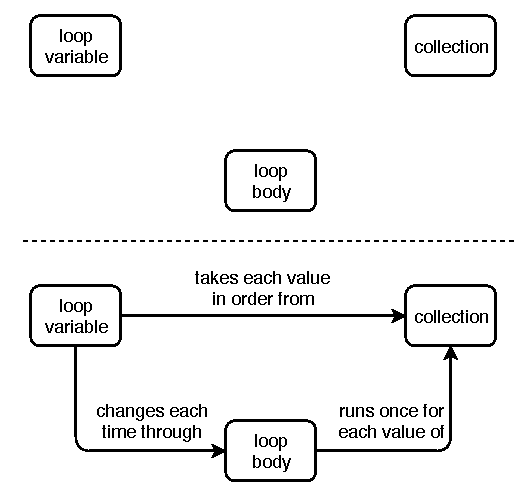
\includegraphics{../docs/fig/for-loop.pdf}
\caption{Concept Map for a For Loop}
\label{f:memory-loop}
\end{figure}

Concept maps can be used in many ways:

\begin{description}

\item[Helping teachers figure out what they're trying to teach.]
  Crucially, a concept map separates content from order: in our
  experience, people rarely wind up teaching things in the order in
  which they first drew them.  (In technical terms, they reduce the
  teacher's cognitive load---we will discuss this again in
  \chapref{s:load}.)

\item[Aiding communication between lesson designers.] Teachers with
  very different ideas of what they're trying to teach are likely to
  pull their learners in different directions; drawing and sharing
  concept maps isn't guaranteed to prevent this, but it helps.

\item[Aiding communication with learners.] While it's possible to give
  learners a pre-drawn map at the start of a lesson for them to
  annotate, it's better to draw it piece by piece while teaching to
  reinforce the ties between what's in the map and what the teacher
  said. (We will return to this idea in
  \secref{s:load-split-attention}.)

\item[For assessment.]  Having learners draw pictures of what they
  think they just heard shows the teacher what they missed and what
  was miscommunicated.  Reviewing learners' concept maps is too
  time-consuming to do as in-class formative assessment, but very
  useful in weekly lectures \emph{once learners are familiar with the
    technique}. The qualification is necessary because any new way of
  doing things initially slows people down---if a student is trying to
  make sense of basic programming, asking them to figure out how to
  draw their thoughts at the same time is an unfair load.

\end{description}

\cite{Kepp2008} looked at the use of concept mapping in computing
education.  One of their findings was that, ``{\ldots}concept mapping
is troublesome for many students because it tests personal
understanding rather than knowledge that was merely learned by rote.''
As someone who values understanding over rote knowledge, I count that
as a benefit.

Some teachers are also skeptical of whether novices can effectively
map their understanding, since introspection and explanation of
understanding are generally more advanced skills than understanding
itself.  Like any other new tool or technique, concept maps have to be
taught and practiced if they are to be effective.

\begin{callout}{Start Anywhere}

  When asked to draw their first concept map, many people will stare
  at the blank page in front of them, not knowing where to start.
  When this happens, right down two words associated with the topic
  you're trying to map, then draw a line between them and add a label
  explaining how those two ideas are related.  You can then ask what
  other things are related in the same way, what parts those things
  have, or what happens before or after the concepts already on the
  page in order to discover more nodes and arcs.  After that, the hard
  part is often stopping.

\end{callout}

Concept maps are just one way to represent our understanding of a
subject; others include mind maps (which are usually radial and
hierarchical), conceptual diagrams (which use predefined categories
and relationships), and visual metaphors (which are striking images
overlaid with text) \cite{Eppl2006}.  Maps, flowcharts, and blueprints
can also be useful in some contexts, as can decision trees like
\cite{Abel2009} that shows how to choose the right kind of chart for
different kinds of questions and data.

What each does is \glossref{g:externalized-cognition}{externalize
  cognition}, i.e., make thought processes and mental models visible
so that they can be compared, contrasted, and combined.
\cite{Cher2007} suggests that externalizing cognition may be the main
reason developers draw diagrams when they are discussing things.  They
found that most developers can't identify the parts of their own
diagrams shortly after having created them---instead of archiving
information for posterity, diagrams are actually a cache for
short-term memory that lets a participant in the discussion point at a
wiggly bubble and say ``that'' to trigger recall of several minutes of
debate.

\begin{callout}{Rough Work and Honesty}

  Many user interface designers believe that it's better to show
  people rough sketches of their ideas rather than polished mock-ups
  because people are more likely to give honest feedback on something
  that they think only took a few minutes to create---if it looks as
  though what they're critiquing took hours to create, most will pull
  their punches.  When drawing concept maps to motivate discussion,
  you should therefore use pencils and scrap paper (or pens and a
  whiteboard) rather than fancy computer drawing tools.

\end{callout}

\section{Seven Plus or Minus Two}\label{s:memory-seven-plus-or-minus}

While the graph model of knowledge is wrong but useful, another simple
model has a sounder physiological basis. As a rough approximation,
human memory can be divided into two distinct layers. The first,
called \glossref{g:long-term-memory}{long-term} or
\glossref{g:persistent-memory}{persistent memory}, is where we store
things like our friends' names, our home address, and what the clown
did at our eighth birthday party that scared us so much. It is
essentially unbounded: barring injury or disease, we will die before
it fills up. However, it is also slow to access---too slow to help us
handle hungry lions and disgruntled family members.

Evolution has therefore given us a second system called
\glossref{g:short-term-memory}{short-term} or
\glossref{g:working-memory}{working memory}. It is much faster, but
also much smaller: \cite{Mill1956} estimated that the average adult's
working memory could only hold $7{\pm}2$ items at a time. This is why
\href{https://www.quora.com/Why-did-Bell-Labs-create-phone-numbers-of-7-digits-10-digits-Is-there-a-reason-that-dashes-and-brackets-are-used}{phone
  numbers} are typically 7 or 8 digits long: back when phones had
dials instead of keypads, that was the longest string of numbers most
adults could remember accurately for as long as it took the dial to go
around several times.  As \secref{s:memory-pattern} discusses,
short-term memory may actually be as small as $4{\pm}1$ items; our
innate tendency to remember things together gives the illusion of it
being larger.

\begin{callout}{Participation}

  The size of working memory is sometimes used to explain why sports
  teams tend to have about half a dozen members or be broken down into
  sub-groups like the forwards and backs in rugby.  It is also used to
  explain why meetings are only productive up to a certain number of
  participants: if twenty people try to discuss something, either
  three meetings are going on at once or half a dozen people are
  talking while everyone else listens.  The argument is that people's
  ability to keep track of their peers is constrained by the size of
  working memory, but so far as I know, the link has never been
  proven.

\end{callout}

$7{\pm}2$ is probably the most important number in programming. When
someone is trying to write the next line of a program, or understand
what's already there, they need to keep a bunch of arbitrary facts
straight in their head: what does this variable represent, what value
does it currently hold, etc. If the number of facts grows too large,
their mental model of the program comes crashing down (something we
have all experienced).

$7{\pm}2$ is also the most important number in teaching. A teacher
cannot push information directly into a learner's long-term memory.
Instead, whatever they present is first stored in the learner's
short-term memory, and is only transferred to long-term memory after
it has been held there and rehearsed
(\secref{s:individual-strategies}).  If the teacher presents too much
information too quickly, the new will displace the old before it has a
chance to consolidate in long-term memory.

This is one of the reasons to create a concept map for a lesson when
designing it: doing so helps the teacher identify how many pieces of
separate information the learner will need to store in memory as the
lesson unfolds.  In practice, I often draw a concept map, realize
there's far too much in it to teach in a single pass, and then carve
out tightly-connected subsections to break the lesson into digestible
pieces, each of which leads to a formative assessment.

\begin{callout}{Building Concept Maps Together}

  Concept maps can be used as a classroom discussion exercise. Put
  learners in small groups (2--4 people each), give each group some
  sticky notes on which a few key concepts are written, and have them
  build a concept map on a whiteboard by placing those sticky notes,
  connecting them with labelled arcs, and adding any other concepts
  they think they need.

  The next time you have a team meeting, give everyone a sheet of
  paper and have them spend a few minutes drawing a concept map of the
  project you're all working on---separately. On the count of three,
  have everyone reveal their concept maps simultaneously. Once
  everyone realizes how different their mental models of the project
  are, a lot of interesting discussion will ensue{\ldots}.

\end{callout}

The simple model of memory presented here has largely been replaced by
a more sophisticated one in which short-term memory is broken down
into several modal stores (e.g., for visual vs.\ linguistic memory),
each of which does some involuntary preprocessing \cite{Mill2016a}.
Our presentation is therefore an example of a mental model that aids
learning and everyday work, but is eventually superseded by something
more complicated.

Research also now indicates that the limiting factor for long-term
memory is not retention, but rather the ability to recall memories
that are present.  Studying in short, spaced periods in a variety of
contexts improves recall; the reason may be that doing so creates more
cues than cramming (\secref{s:individual-strategies}).

\section{Pattern Recognition}\label{s:memory-pattern}

The preceding section said that short-term memory can only store
$7{\pm}2$ items at a time, and recent research have suggested that its
actual size might be as low as $4{\pm}1$ items \cite{Dida2016}.  In
order to handle larger information sets, our minds create
\glossref{g:chunking}{chunks}. For example, most of us remember words
as single items, rather than as sequences of letters. Similarly, the
pattern made by five spots on cards or dice is remembered as a whole
rather than as five separate pieces of information.

One key finding in cognition research is that experts have more and
larger chunks than non-experts, i.e., experts ``see'' larger patterns,
and have more patterns to match things against. This allows them to
reason at a higher level, and to search for information more quickly
and more accurately.  However, chunking can also mislead us if we
mis-identify things: newcomers really can sometimes see things that
experts have looked at and missed.

Given how important chunking is to thinking, it is tempting to try to
teach patterns directly.  One way to do this is to identify
\href{https://en.wikipedia.org/wiki/Software_design_pattern}{design
  patterns}, which are reusable solutions to common problems. Patterns
help competent practitioners think and talk to each other in many
domains (including teaching \cite{Berg2012}), but pattern catalogs are
too dry and too abstract for novices to make sense of on their own.
That said, giving names to a small number of patterns does seem to
help with teaching, primarily by giving the learners a richer
vocabulary to think and communicate with
\cite{Kuit2004,Byck2005,Saja2006}.  We will return to this in
\secref{s:pck-programming}.

\section{Becoming an Expert}\label{s:memory-becoming-expert}

So how does someone become an expert?  The idea that ten thousand
hours of practice will do it is widely quoted but
\href{http://www.goodlifeproject.com/podcast/anders-ericsson/}{probably
  not true}: doing the same thing over and over again is much more
likely to solidify bad habits than improve performance. What actually
works is \glossref{g:deliberate-practice}{deliberate practice} (also
sometimes called \glossref{g:reflective-practice}{reflective
  practice}), which is doing similar but subtly different things,
paying attention to what works and what doesn't, and then changing
behavior in response to that feedback to get cumulatively better.

A common progression is for people to go through three stages:

\begin{description}

  \item[Act on feedback from others.]  For example, a student might
    write an essay about what they did on their summer holiday and get
    feedback from a teacher telling them how to improve it.

  \item[Give feedback to others.] For example, they might critique
    character development in \emph{The Catcher in the Rye}.  For this
    to be effective, it's essential that they get feedback on their
    feedback, i.e., that the teacher critique their analysis.

  \item[Give feedback to themselves.]  At some point, they start
    critiquing their own work in real time (or nearly so) using the
    skills they have now built up. Doing this is so much faster than
    waiting for feedback from others that proficiency suddenly starts
    to take off.

\end{description}

\begin{callout}{What Counts as Deliberate Practice?}

  \cite{Macn2014} found that ``{\ldots}deliberate practice explained
  26\% of the variance in performance for games, 21\% for music, 18\%
  for sports, 4\% for education, and less than 1\% for professions.''
  However, \cite{Eric2016} critiqued this finding by saying, ``Summing
  up every hour of any type of practice during an individual's career
  implies that the impact of all types of practice activity on
  performance is equal---an assumption that{\ldots}is inconsistent with
  the evidence.''  To be effective, deliberate practice requires both
  a clear performance goal and immediate informative feedback.

\end{callout}

\section{Exercises}\label{s:memory-exercises}

\exercise{Concept Mapping}{pairs}{30}

Draw a concept map for something you would teach in five minutes.
Trade with a partner, and critique each other's maps. Do they present
concepts or surface detail?  Which of the relationships in your
partner's map do you consider concepts and vice versa?

\exercise{Concept Mapping (Again)}{small groups}{20}

Working in groups of 3--4, have each person independently draw a
concept map showing their mental model of what goes on in a classroom.
When everyone is done, compare the concept maps.  Which concepts and
relationships are common?  Which are different?  Where do your mental
models agree and disagree?

\exercise{A Concept Map for This Material}{individual}{30}

After you have finished going through this material (not just this
chapter), pick one small topic, draw a concept map for it, and send it
to us (\appref{s:joining}).  If we decide to add it to this book, we
will add you to the credits in the introduction.

\exercise{Noticing Your Blind Spot}{small groups}{10}

Consider all the things you have to know to understand this one line of
Python source code:

\begin{verbatim}
answers = ['tuatara', 'tuataras', 'bus', "lick"]
\end{verbatim}

\noindent
As \href{https://twitter.com/elliewix/status/981285432922202113}{Elizabeth Wickes points out}:

\begin{itemize}

\item
  The square brackets surrounding the content mean we're working with
  a list (as opposed to square brackets immediately to the right of
  something, which is a data extraction notation).

\item
  The elements are separated by commas, which are outside/between the
  quotes (rather than inside, as they would be for quoted speech).

\item
  Each element is a character string, and we know that because of the
  quotes. We could have number or other data types in here if we
  wanted; we need quotes because we're working with strings.

\item
  We're mixing our use of single and double quotes, and Python doesn't
  care (so long as they balance around the individual strings).

\item
  Each comma is followed by a space, which is not required by Python,
  but we prefer it for readability.

\end{itemize}

\noindent
Each of these details might be overlooked by an expert.  Working in
groups of 3--4, select something equally short from a lesson you have
recently taught or taken and break it down to this level of detail.
